
\section{A 4 plot slide}
\begin{frame}{A 4 plot slide}
Some top text
\begin{columns}
\begin{column}{0.4\textwidth}
\begin{center}
Optional title
\\
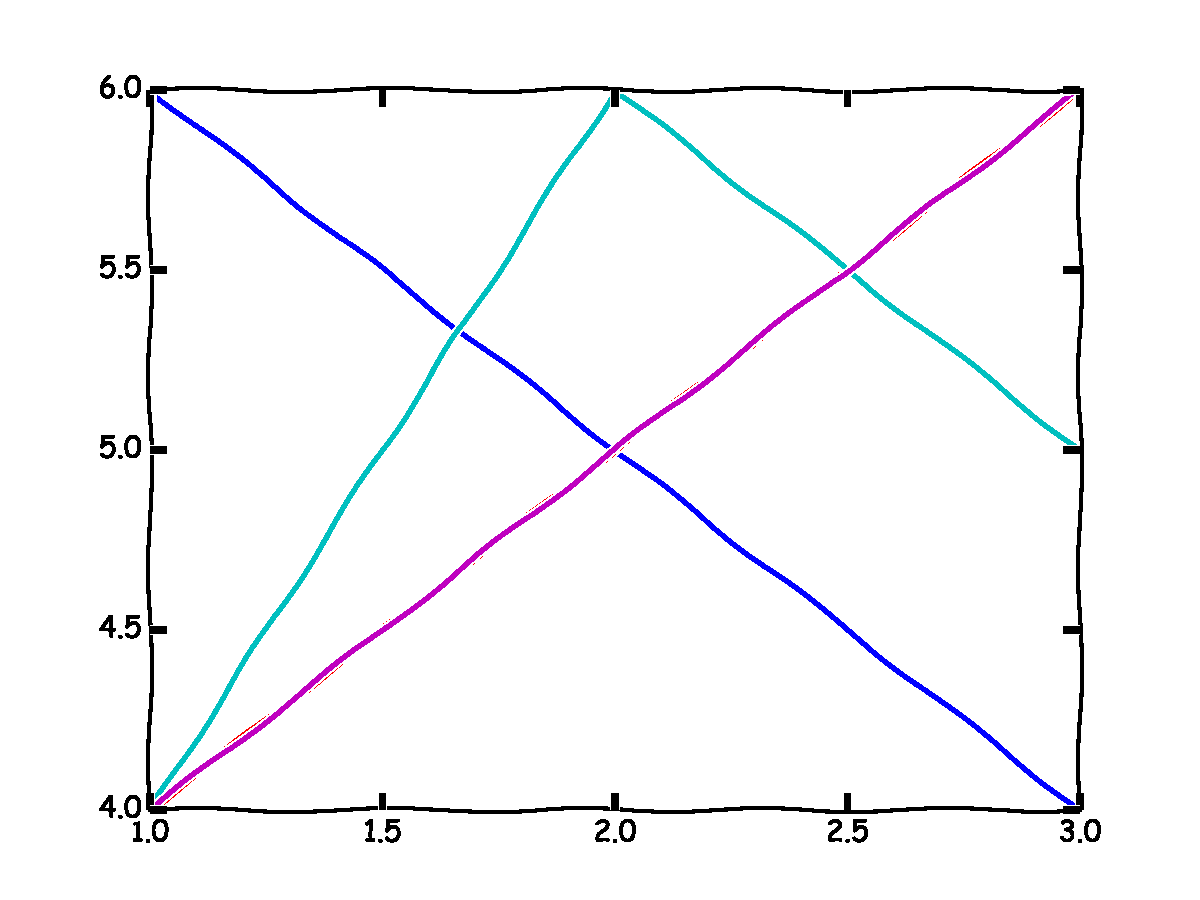
\includegraphics[width=\textwidth]{example/plot1.pdf}
\\
Plot 3 title
\\
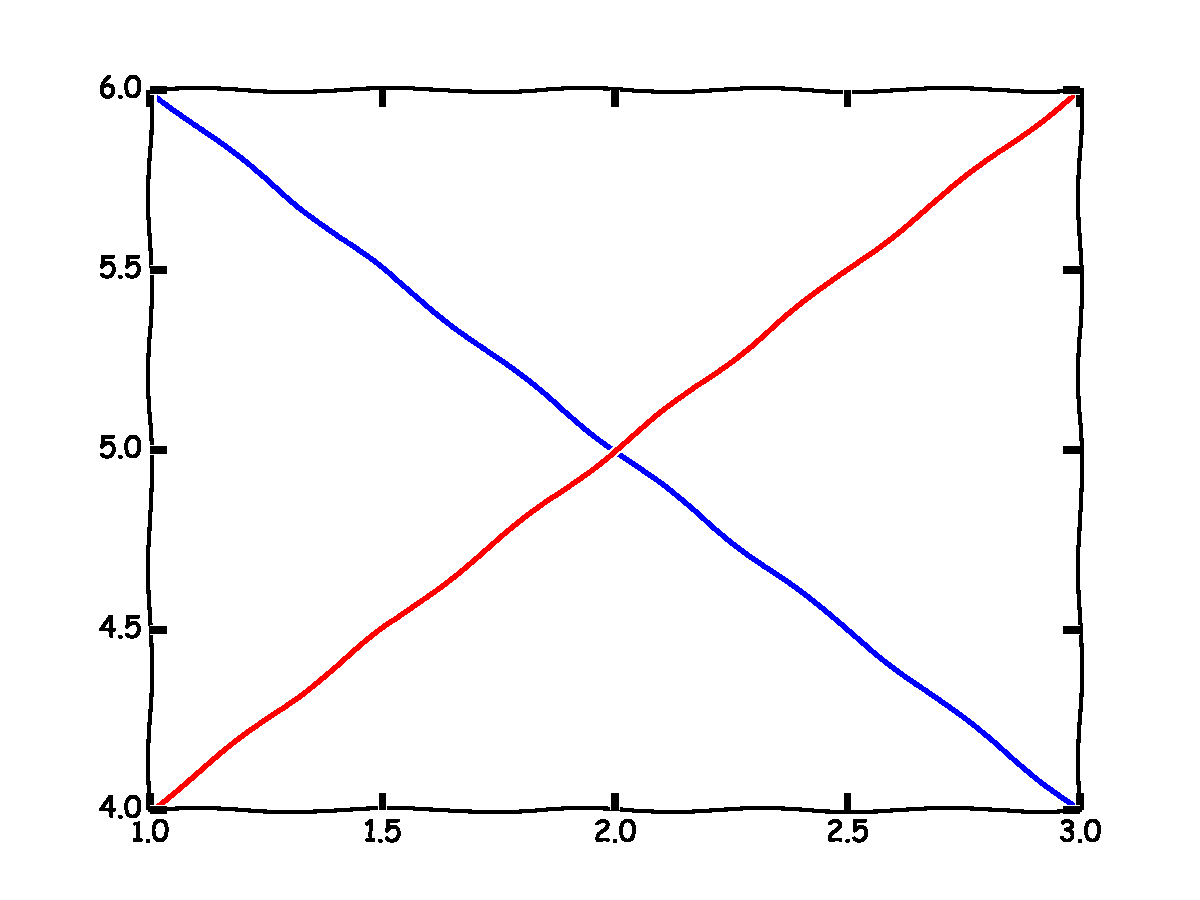
\includegraphics[width=\textwidth]{example/plot3.pdf}
\\
\end{center}
\end{column}

\begin{column}{0.4\textwidth}
\begin{center}
Plot 2 title
\\
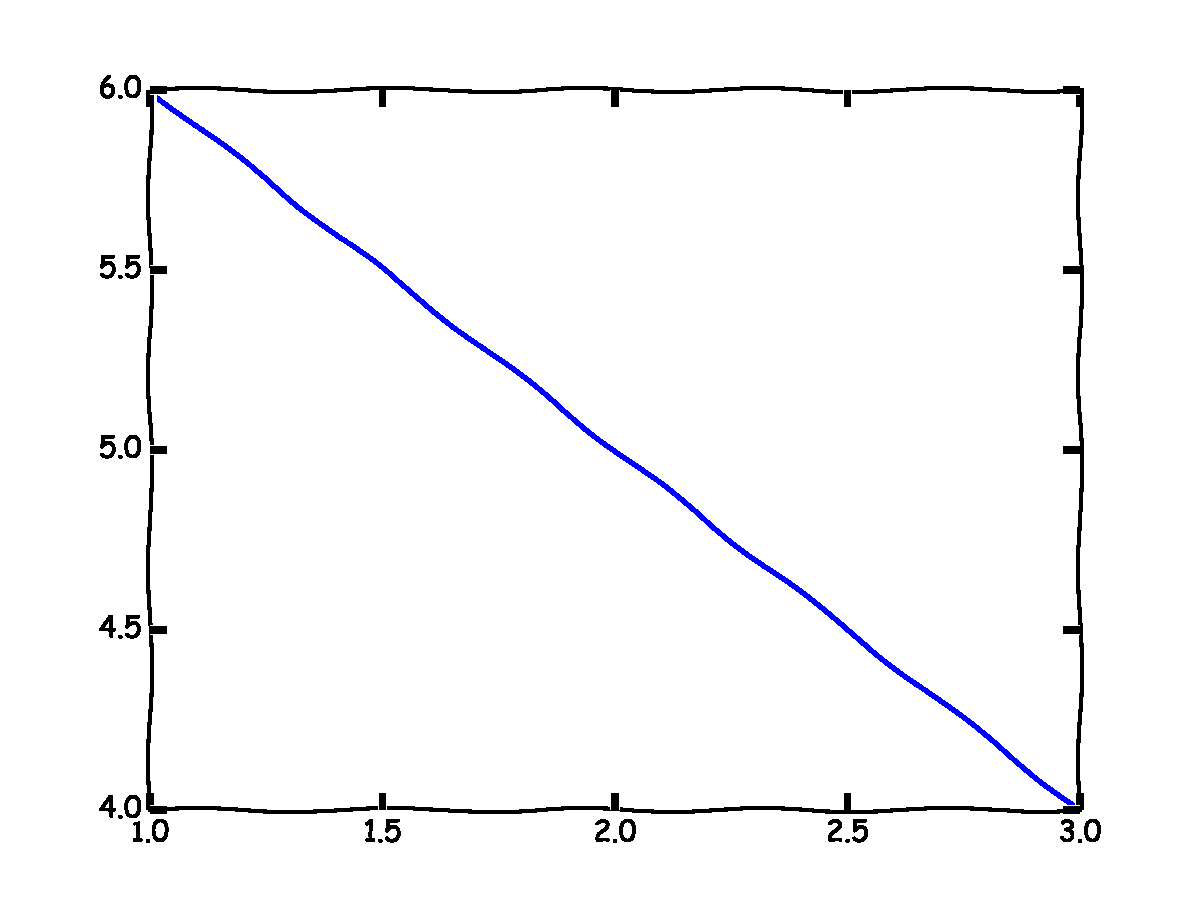
\includegraphics[width=\textwidth]{example/plot2.pdf}
\\
Plot 4 title
\\
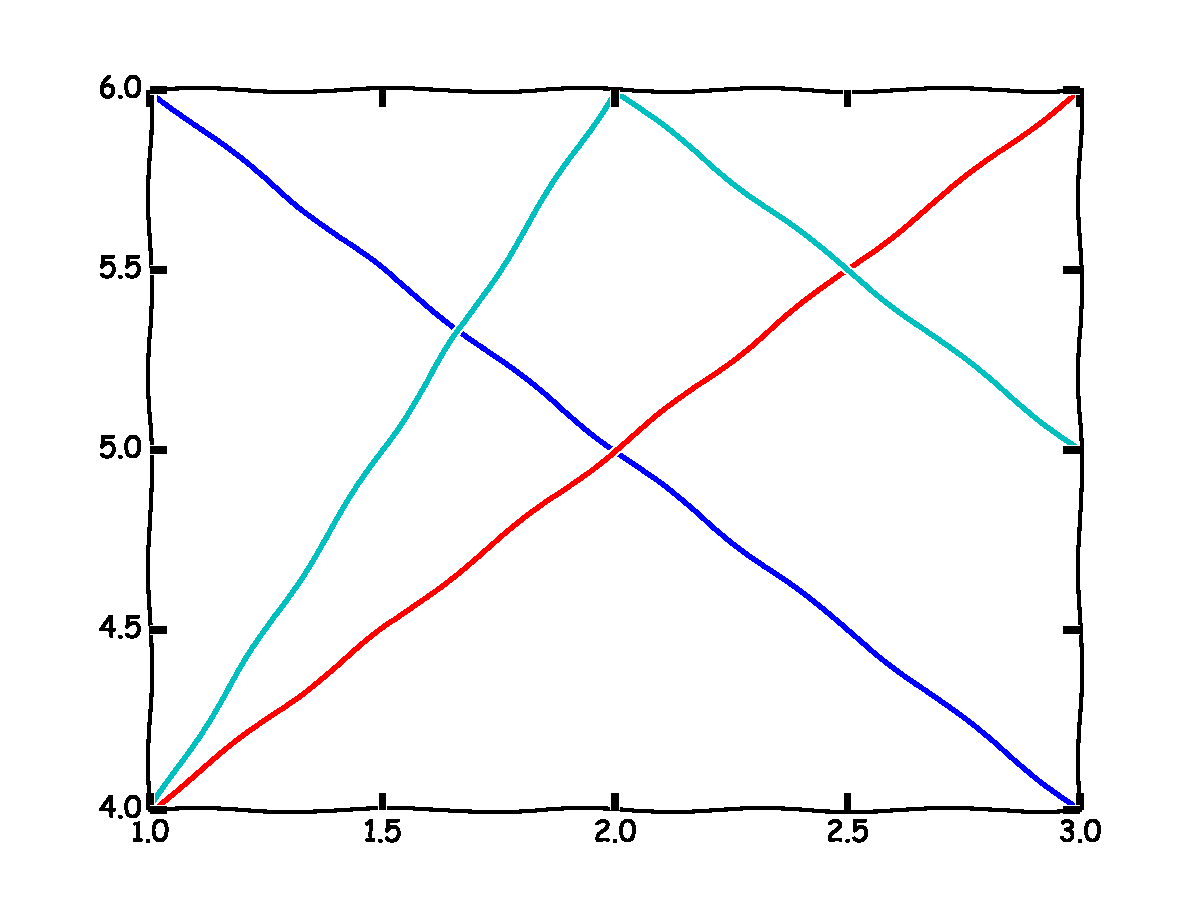
\includegraphics[width=\textwidth]{example/plot4.pdf}
\\
\end{center}
\end{column}
\end{columns}
Some bottom text
\end{frame}

\section{Two plot slide}
\begin{frame}{Two plot slide}
With no plot titles
\begin{columns}
\begin{column}{0.5\textwidth}
\begin{center}
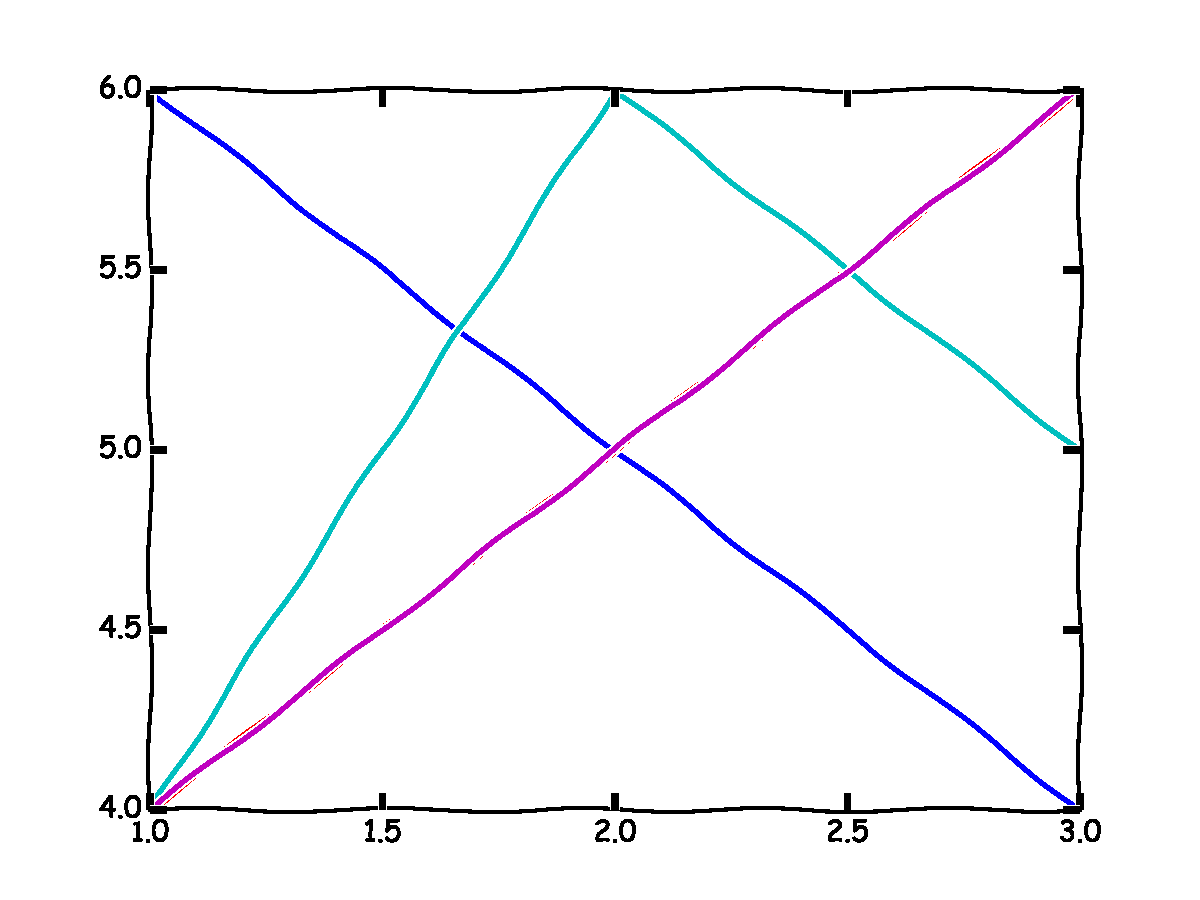
\includegraphics[width=\textwidth]{example/plot1.pdf}
\\
\end{center}
\end{column}

\begin{column}{0.5\textwidth}
\begin{center}
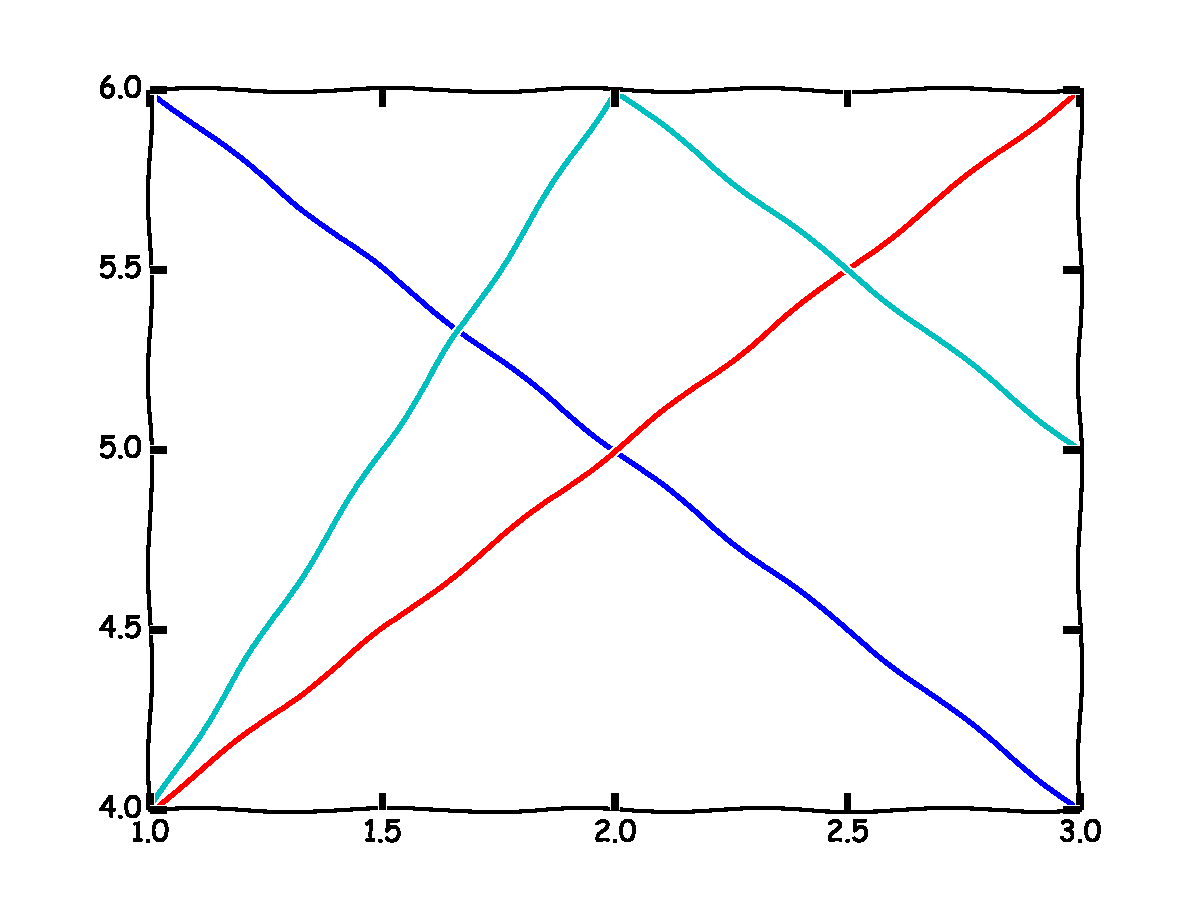
\includegraphics[width=\textwidth]{example/plot4.pdf}
\end{center}
\end{column}
\end{columns}
blah blah blah
\end{frame}

\section{Simple one plot slide}
\begin{frame}{Simple one plot slide}
Some top text
\begin{center}
Optional title
\\
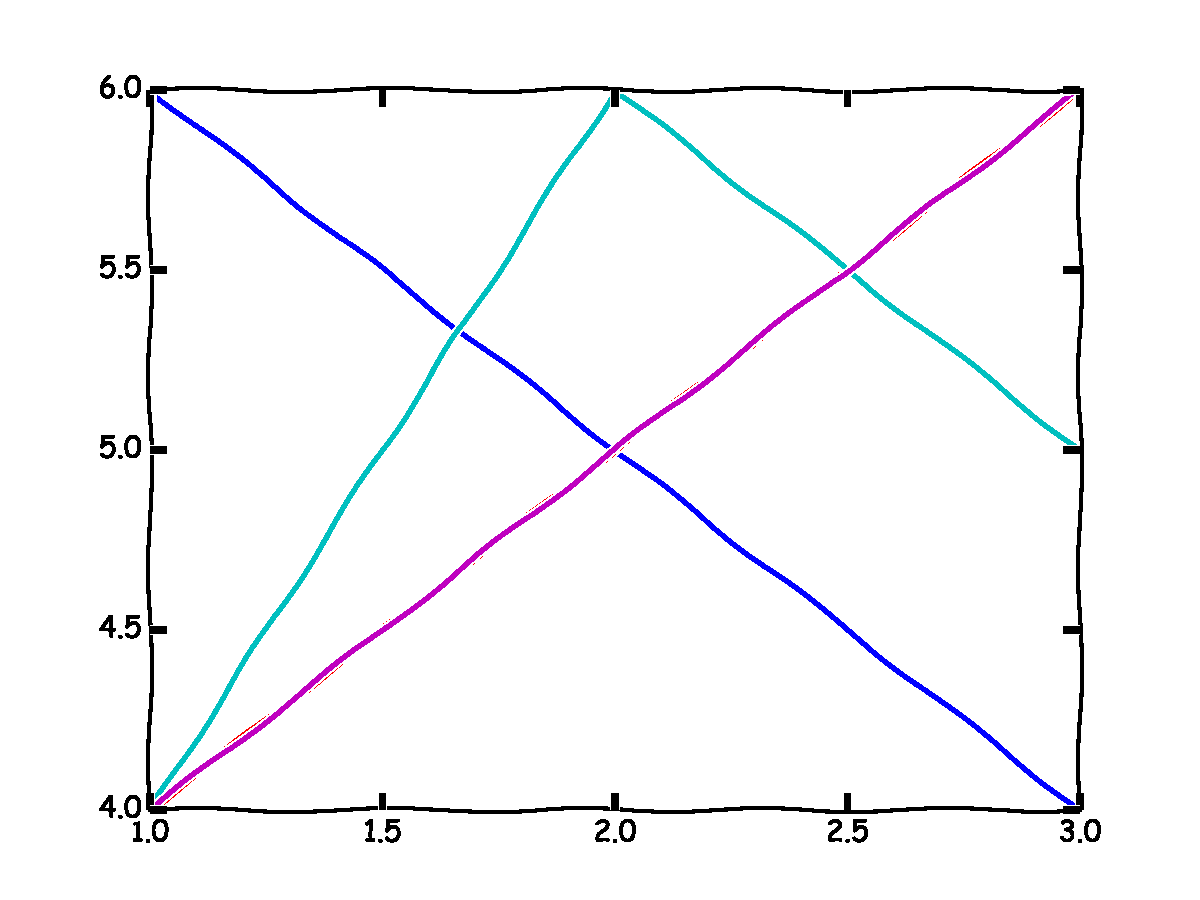
\includegraphics[width=0.8\textwidth]{example/plot1.pdf}
\\
\end{center}
Some bottom text
\end{frame}

\section{A whopping 6 plots}
\begin{frame}{A whopping 6 plots}
Are you crazy
\begin{columns}
\begin{column}{0.33\textwidth}
\begin{center}
Optional title
\\
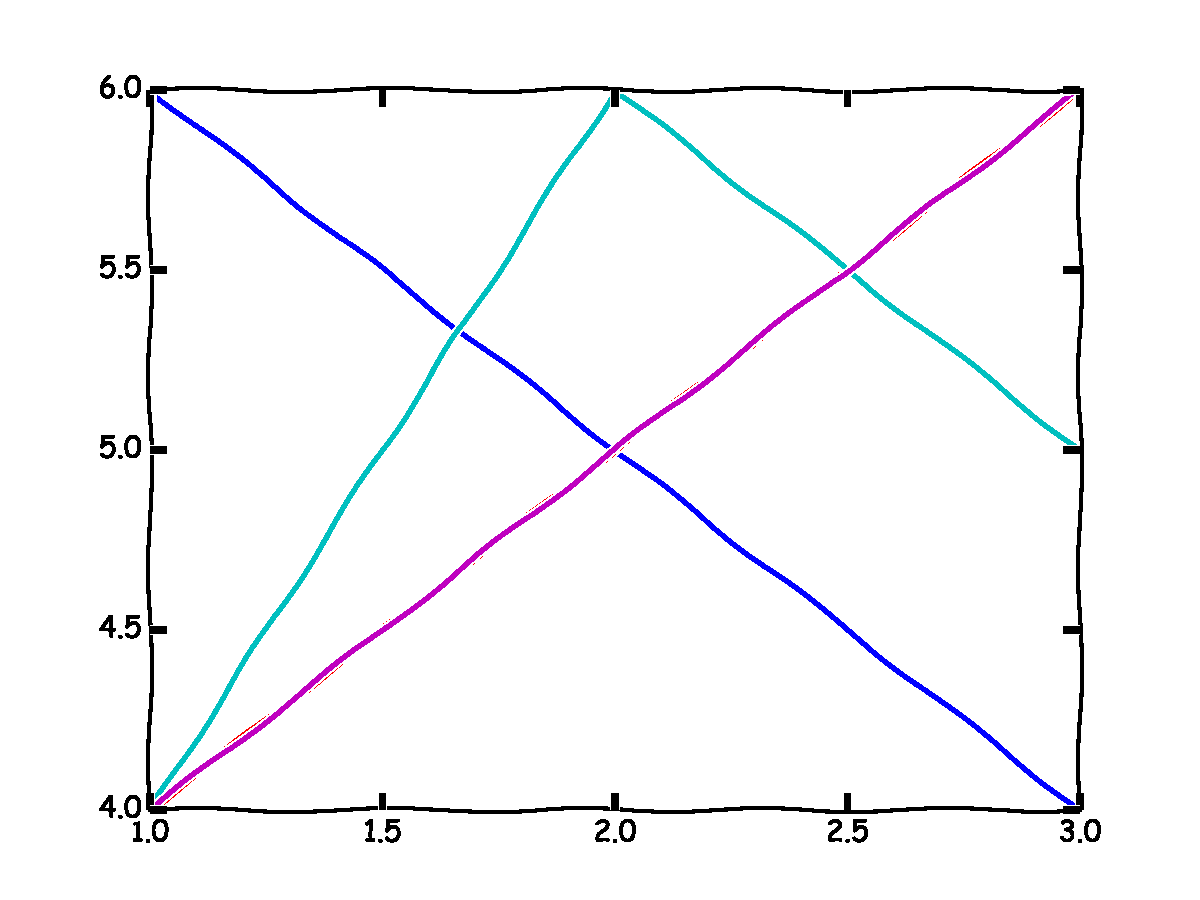
\includegraphics[width=\textwidth]{example/plot1.pdf}
\\
Plot 4 title
\\
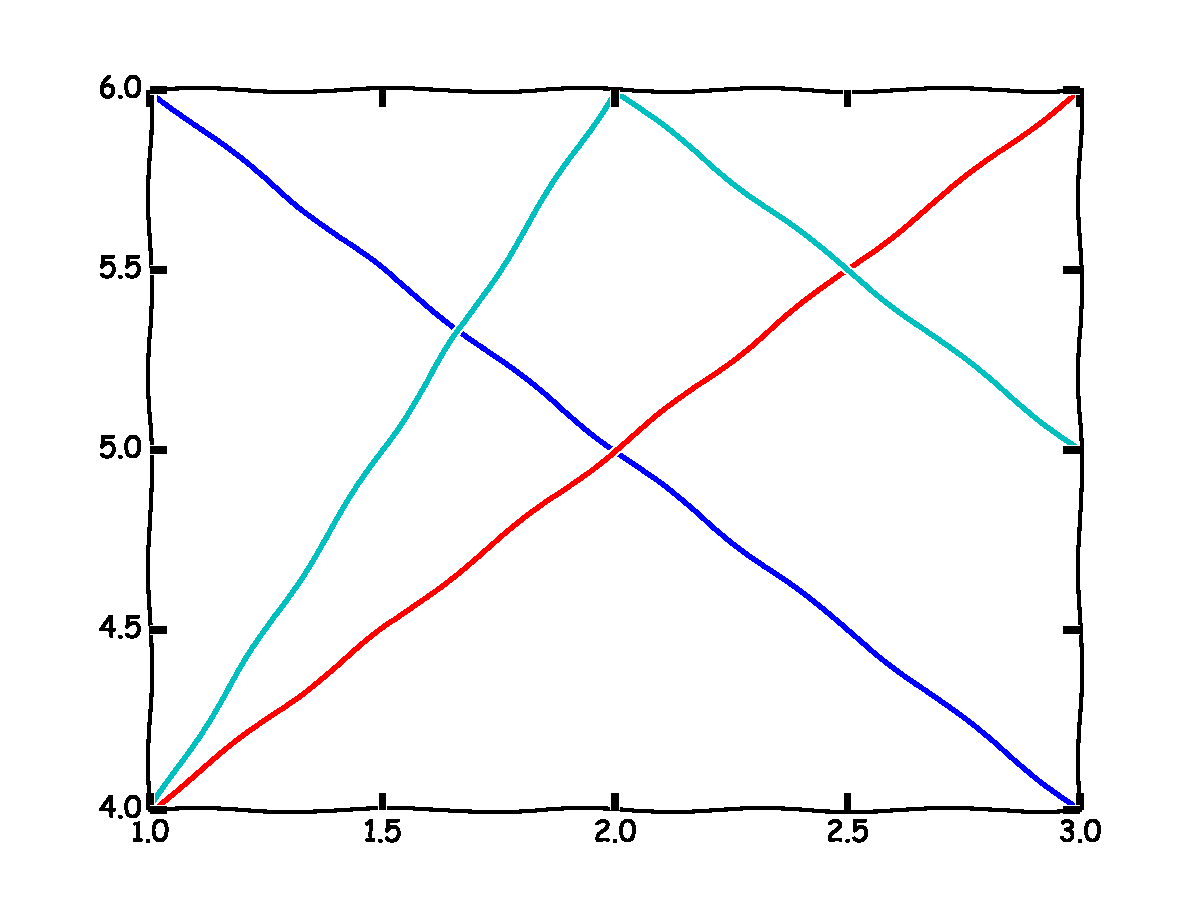
\includegraphics[width=\textwidth]{example/plot4.pdf}
\end{center}
\end{column}

\begin{column}{0.33\textwidth}
\begin{center}
Plot 2 title
\\
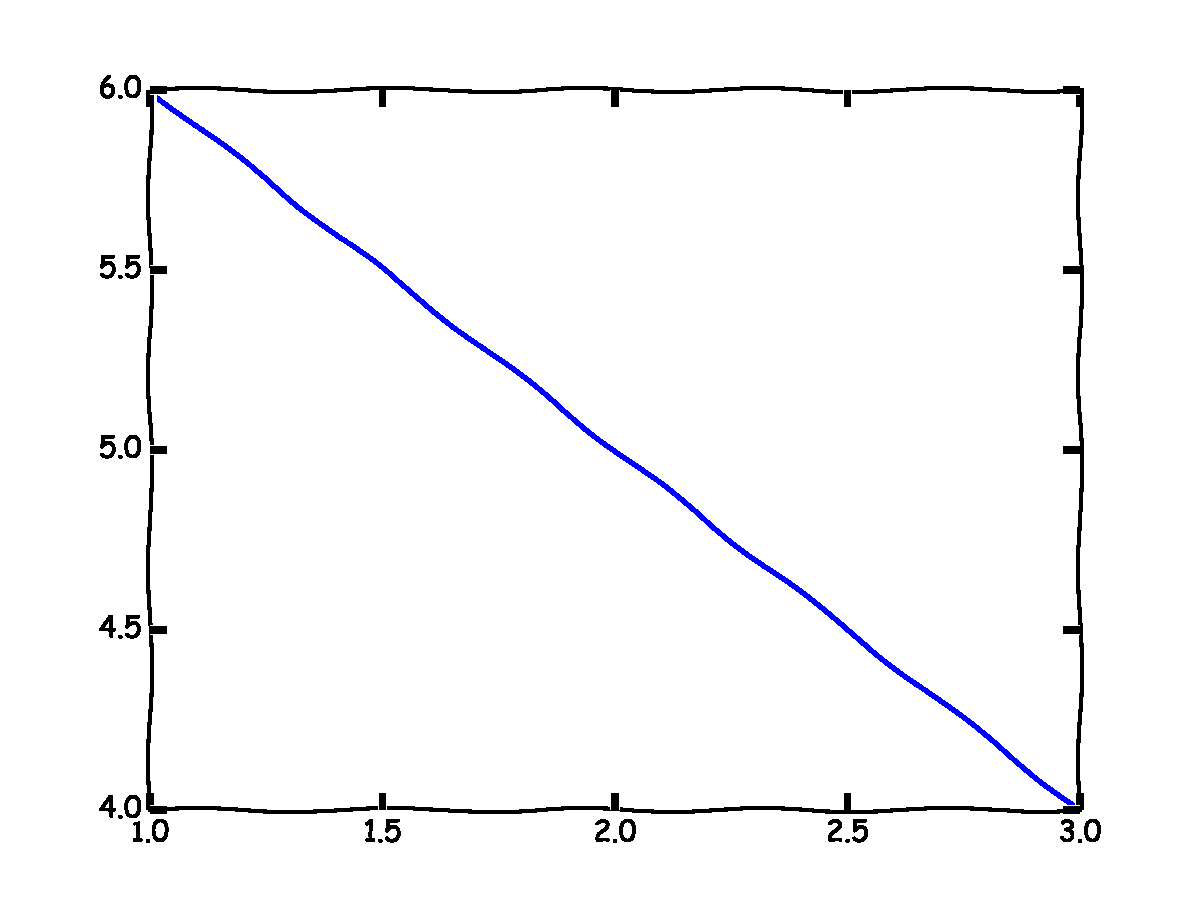
\includegraphics[width=\textwidth]{example/plot2.pdf}
\\
Plot 5 title
\\
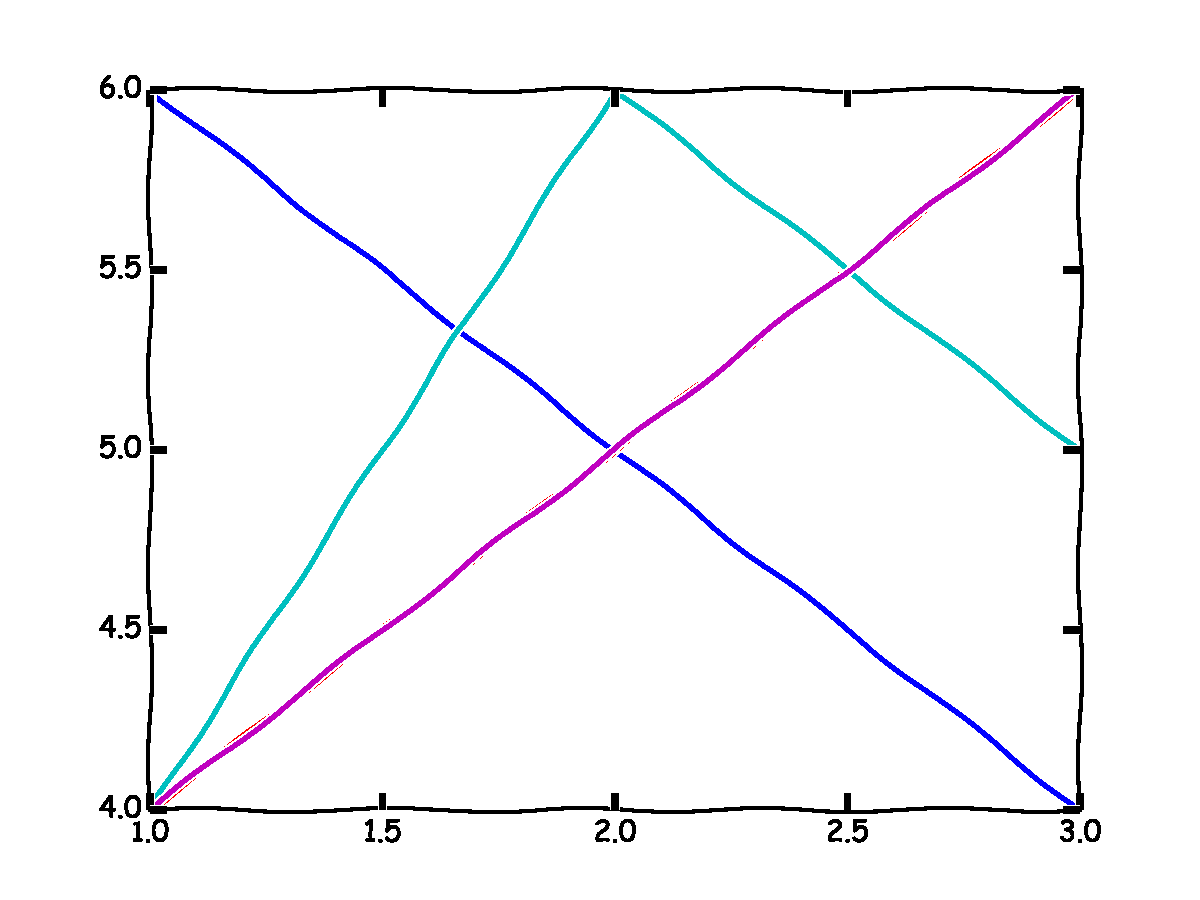
\includegraphics[width=\textwidth]{example/plot1.pdf}
\end{center}
\end{column}

\begin{column}{0.33\textwidth}
\begin{center}
Plot 3 title
\\
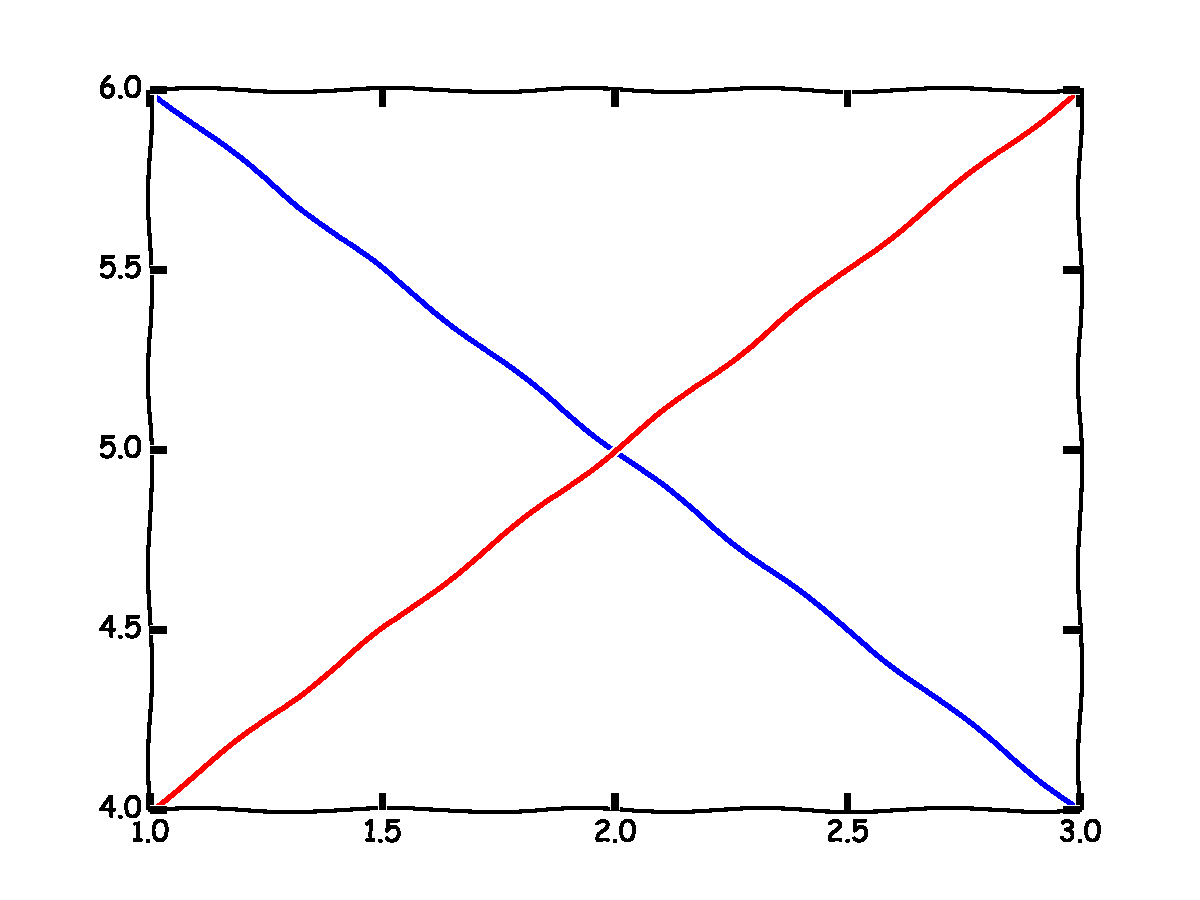
\includegraphics[width=\textwidth]{example/plot3.pdf}
\\
Plot 6 title
\\
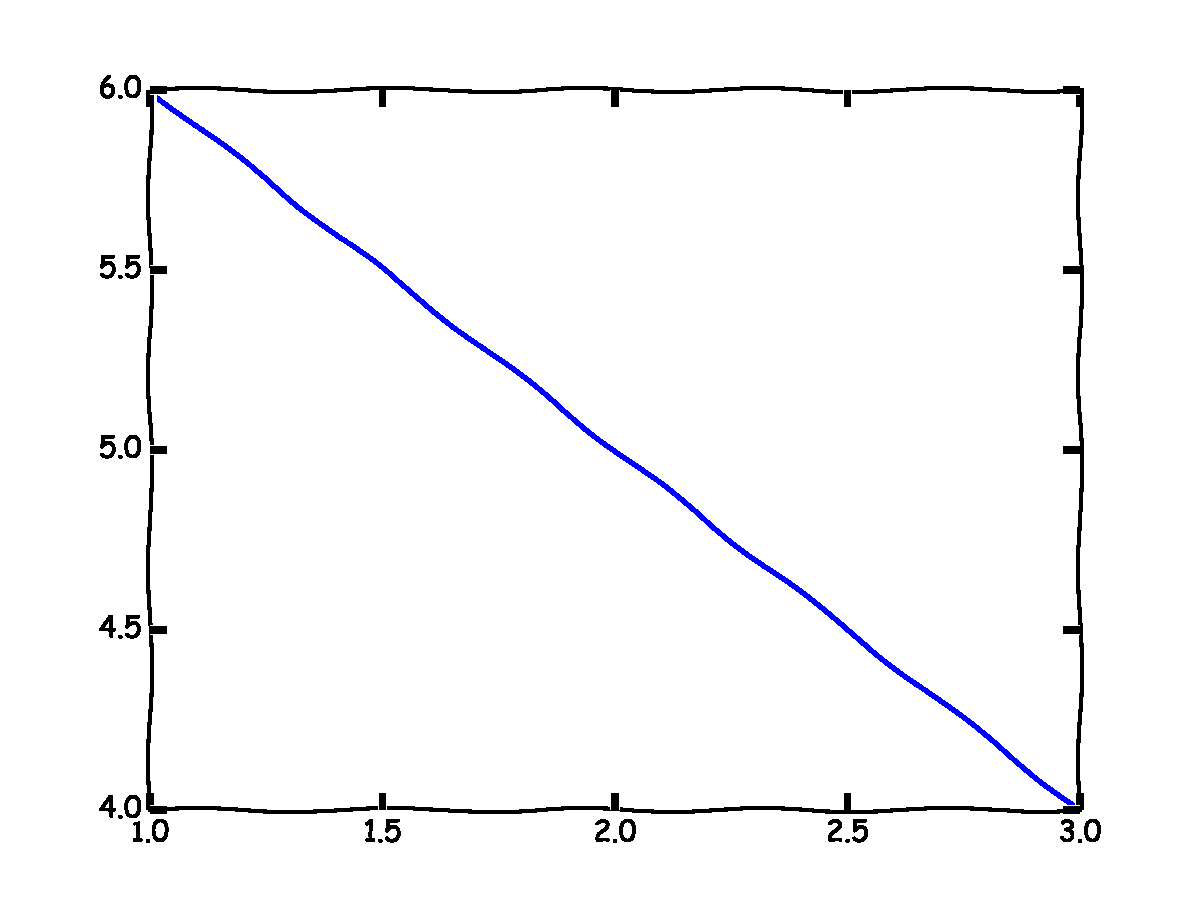
\includegraphics[width=\textwidth]{example/plot2.pdf}
\end{center}
\end{column}
\end{columns}
Some bottom text
\end{frame}
